\hypertarget{convll_8h}{
\section{convll.h File Reference}
\label{convll_8h}\index{convll.h@{convll.h}}
}
{\tt \#include $<$stdio.h$>$}\par
{\tt \#include $<$stdlib.h$>$}\par
{\tt \#include \char`\"{}bit\-Set.h\char`\"{}}\par


Include dependency graph for convll.h:\begin{figure}[H]
\begin{center}
\leavevmode
\includegraphics[width=130pt]{convll_8h__incl}
\end{center}
\end{figure}


This graph shows which files directly or indirectly include this file:\begin{figure}[H]
\begin{center}
\leavevmode
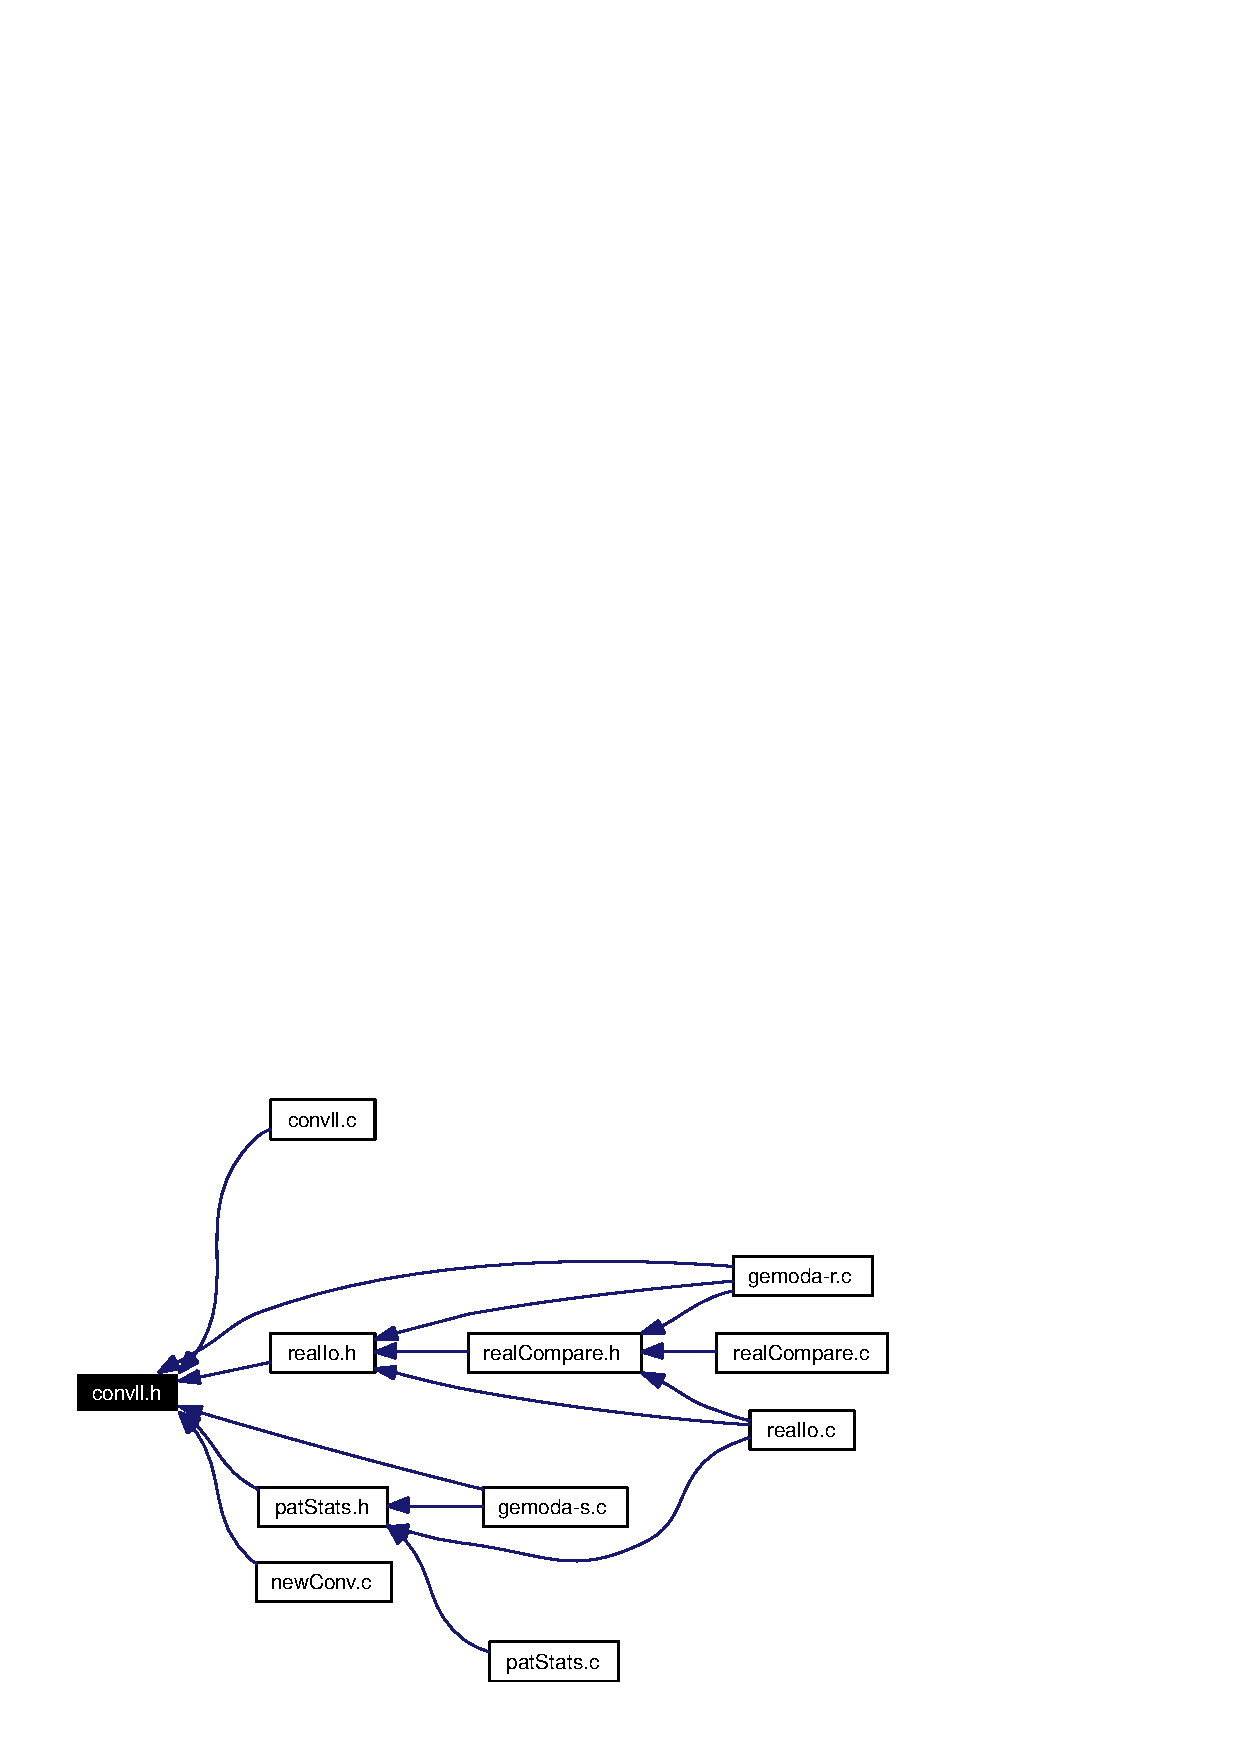
\includegraphics[width=213pt]{convll_8h__dep__incl}
\end{center}
\end{figure}
\subsection*{Data Structures}
\begin{CompactItemize}
\item 
struct \hyperlink{structcSet__t}{c\-Set\_\-t}
\item 
struct \hyperlink{structcnode}{cnode}
\item 
struct \hyperlink{structmnode}{mnode}
\end{CompactItemize}
\subsection*{Typedefs}
\begin{CompactItemize}
\item 
typedef \hyperlink{structcnode}{cnode} \hyperlink{convll_8h_a0}{cll\_\-t}
\item 
typedef \hyperlink{structmnode}{mnode} \hyperlink{convll_8h_a1}{mll\_\-t}
\end{CompactItemize}
\subsection*{Functions}
\begin{CompactItemize}
\item 
\hyperlink{structcnode}{cll\_\-t} $\ast$ \hyperlink{convll_8h_a2}{push\-Cll} (\hyperlink{structcnode}{cll\_\-t} $\ast$head)
\item 
\hyperlink{structcnode}{cll\_\-t} $\ast$ \hyperlink{convll_8h_a3}{pop\-Cll} (\hyperlink{structcnode}{cll\_\-t} $\ast$head)
\item 
\hyperlink{structcnode}{cll\_\-t} $\ast$ \hyperlink{convll_8h_a4}{pop\-All\-Cll} (\hyperlink{structcnode}{cll\_\-t} $\ast$head)
\item 
int \hyperlink{convll_8h_a5}{print\-Cll} (\hyperlink{structcnode}{cll\_\-t} $\ast$head)
\item 
\hyperlink{structcnode}{cll\_\-t} $\ast$ \hyperlink{convll_8h_a6}{inithead\-Cll} (\hyperlink{structcnode}{cll\_\-t} $\ast$head, \hyperlink{structcSet__t}{c\-Set\_\-t} $\ast$newset)
\item 
\hyperlink{structcnode}{cll\_\-t} $\ast$ \hyperlink{convll_8h_a7}{pushc\-Set} (\hyperlink{structcnode}{cll\_\-t} $\ast$head, \hyperlink{structcSet__t}{c\-Set\_\-t} $\ast$newset)
\item 
\hyperlink{structcnode}{cll\_\-t} $\ast$ \hyperlink{convll_8h_a8}{push\-Clique} (\hyperlink{structbitSet__t}{bit\-Set\_\-t} $\ast$clique, \hyperlink{structcnode}{cll\_\-t} $\ast$head, int $\ast$index\-To\-Seq, int p)
\item 
\hyperlink{structmnode}{mll\_\-t} $\ast$ \hyperlink{convll_8h_a9}{push\-Mem\-Stack} (\hyperlink{structmnode}{mll\_\-t} $\ast$head, int clique\-Num)
\item 
\hyperlink{structmnode}{mll\_\-t} $\ast$ \hyperlink{convll_8h_a10}{pop\-Mem\-Stack} (\hyperlink{structmnode}{mll\_\-t} $\ast$head)
\item 
\hyperlink{structmnode}{mll\_\-t} $\ast$ \hyperlink{convll_8h_a11}{pop\-Whole\-Mem\-Stack} (\hyperlink{structmnode}{mll\_\-t} $\ast$head)
\item 
\hyperlink{structmnode}{mll\_\-t} $\ast$$\ast$ \hyperlink{convll_8h_a12}{add\-To\-Stacks} (\hyperlink{structcnode}{cll\_\-t} $\ast$node, \hyperlink{structmnode}{mll\_\-t} $\ast$$\ast$member\-Stacks)
\item 
\hyperlink{structmnode}{mll\_\-t} $\ast$$\ast$ \hyperlink{convll_8h_a13}{fill\-Member\-Stacks} (\hyperlink{structcnode}{cll\_\-t} $\ast$head, \hyperlink{structmnode}{mll\_\-t} $\ast$$\ast$member\-Stacks)
\item 
\hyperlink{structmnode}{mll\_\-t} $\ast$$\ast$ \hyperlink{convll_8h_a14}{empty\-Member\-Stacks} (\hyperlink{structmnode}{mll\_\-t} $\ast$$\ast$member\-Stacks, int size)
\item 
void \hyperlink{convll_8h_a15}{print\-Member\-Stacks} (\hyperlink{structmnode}{mll\_\-t} $\ast$$\ast$member\-Stacks, int size)
\item 
\hyperlink{structbitSet__t}{bit\-Set\_\-t} $\ast$ \hyperlink{convll_8h_a16}{search\-Mems\-With\-List} (int $\ast$list, int listsize, \hyperlink{structmnode}{mll\_\-t} $\ast$$\ast$mem\-List, int num\-Offsets, \hyperlink{structbitSet__t}{bit\-Set\_\-t} $\ast$queue)
\item 
\hyperlink{structbitSet__t}{bit\-Set\_\-t} $\ast$ \hyperlink{convll_8h_a17}{set\-Stack\-True} (\hyperlink{structmnode}{mll\_\-t} $\ast$$\ast$mem\-List, int i, \hyperlink{structbitSet__t}{bit\-Set\_\-t} $\ast$queue)
\item 
\hyperlink{structcnode}{cll\_\-t} $\ast$ \hyperlink{convll_8h_a18}{single\-Clique\-Conv} (\hyperlink{structcnode}{cll\_\-t} $\ast$head, int first\-Clique, \hyperlink{structcnode}{cll\_\-t} $\ast$$\ast$first\-Guess, int second\-Clique, \hyperlink{structcnode}{cll\_\-t} $\ast$$\ast$second\-Guess, \hyperlink{structcnode}{cll\_\-t} $\ast$next\-Phase, \hyperlink{structbitSet__t}{bit\-Set\_\-t} $\ast$print\-Status, int support)
\item 
\hyperlink{structmnode}{mll\_\-t} $\ast$ \hyperlink{convll_8h_a19}{merge\-Intersect} (\hyperlink{structcnode}{cll\_\-t} $\ast$first, \hyperlink{structcnode}{cll\_\-t} $\ast$second, \hyperlink{structmnode}{mll\_\-t} $\ast$intersection, \hyperlink{structbitSet__t}{bit\-Set\_\-t} $\ast$print\-Status, int $\ast$new\-Support)
\item 
\hyperlink{structcnode}{cll\_\-t} $\ast$ \hyperlink{convll_8h_a20}{push\-Conv\-Clique} (\hyperlink{structmnode}{mll\_\-t} $\ast$clique, \hyperlink{structcnode}{cll\_\-t} $\ast$head)
\item 
\hyperlink{structcSet__t}{c\-Set\_\-t} $\ast$ \hyperlink{convll_8h_a21}{mll\-To\-CSet} (\hyperlink{structmnode}{mll\_\-t} $\ast$clique)
\item 
\hyperlink{structcSet__t}{c\-Set\_\-t} $\ast$ \hyperlink{convll_8h_a22}{bit\-Set\-To\-CSet} (\hyperlink{structbitSet__t}{bit\-Set\_\-t} $\ast$clique)
\item 
\hyperlink{structcnode}{cll\_\-t} $\ast$ \hyperlink{convll_8h_a23}{whole\-Clique\-Conv} (\hyperlink{structcnode}{cll\_\-t} $\ast$head, \hyperlink{structcnode}{cll\_\-t} $\ast$node, \hyperlink{structcnode}{cll\_\-t} $\ast$$\ast$first\-Guess, \hyperlink{structmnode}{mll\_\-t} $\ast$$\ast$mem\-List, int num\-Offsets, \hyperlink{structcnode}{cll\_\-t} $\ast$next\-Phase, \hyperlink{structbitSet__t}{bit\-Set\_\-t} $\ast$print\-Status, int support)
\item 
\hyperlink{structcnode}{cll\_\-t} $\ast$ \hyperlink{convll_8h_a24}{whole\-Round\-Conv} (\hyperlink{structcnode}{cll\_\-t} $\ast$$\ast$head, \hyperlink{structmnode}{mll\_\-t} $\ast$$\ast$mem\-List, int num\-Offsets, int support, int length, \hyperlink{structcnode}{cll\_\-t} $\ast$$\ast$all\-Cliques)
\item 
\hyperlink{structcnode}{cll\_\-t} $\ast$ \hyperlink{convll_8h_a25}{complete\-Conv} (\hyperlink{structcnode}{cll\_\-t} $\ast$$\ast$head, int support, int num\-Offsets, int min\-Length, int $\ast$index\-To\-Seq, int p)
\item 
int \hyperlink{convll_8h_a26}{print\-Cll\-Pattern} (\hyperlink{structcnode}{cll\_\-t} $\ast$node, int length)
\item 
int \hyperlink{convll_8h_a27}{uniq\-Clique} (\hyperlink{structcSet__t}{c\-Set\_\-t} $\ast$clique, \hyperlink{structcnode}{cll\_\-t} $\ast$head)
\item 
\hyperlink{structcnode}{cll\_\-t} $\ast$ \hyperlink{convll_8h_a28}{swap\-Nodec\-Set} (\hyperlink{structcnode}{cll\_\-t} $\ast$head, int node, \hyperlink{structcSet__t}{c\-Set\_\-t} $\ast$new\-Clique)
\item 
int \hyperlink{convll_8h_a29}{yank\-Cll} (\hyperlink{structcnode}{cll\_\-t} $\ast$$\ast$head, \hyperlink{structcnode}{cll\_\-t} $\ast$prev, \hyperlink{structcnode}{cll\_\-t} $\ast$$\ast$curr, \hyperlink{structcnode}{cll\_\-t} $\ast$$\ast$all\-Cliques, int length)
\item 
\hyperlink{structcnode}{cll\_\-t} $\ast$ \hyperlink{convll_8h_a30}{remove\-Supers} (\hyperlink{structcnode}{cll\_\-t} $\ast$head, int node, \hyperlink{structcSet__t}{c\-Set\_\-t} $\ast$new\-Clique)
\end{CompactItemize}


\subsection*{Detailed Description}
This header file contains declarations and definitions for dealing with different kinds of sets that are used throughout the convolution stage of Gemoda.

Definition in file \hyperlink{convll_8h-source}{convll.h}.

\subsection*{Typedef Documentation}
\hypertarget{convll_8h_a0}{
\index{convll.h@{convll.h}!cll_t@{cll\_\-t}}
\index{cll_t@{cll\_\-t}!convll.h@{convll.h}}
\subsubsection[cll\_\-t]{\setlength{\rightskip}{0pt plus 5cm}typedef struct \hyperlink{structcnode}{cnode}  \hyperlink{structcnode}{cll\_\-t}}}
\label{convll_8h_a0}


This data structure is a linked list for storing cliques. Each member of the linked list has a set, an ID number, a length (which gives the number of characters in the motif), a pointer to the next member of the linked list, and a floating-point number for storing statistical information.\hypertarget{convll_8h_a1}{
\index{convll.h@{convll.h}!mll_t@{mll\_\-t}}
\index{mll_t@{mll\_\-t}!convll.h@{convll.h}}
\subsubsection[mll\_\-t]{\setlength{\rightskip}{0pt plus 5cm}typedef struct \hyperlink{structmnode}{mnode}  \hyperlink{structmnode}{mll\_\-t}}}
\label{convll_8h_a1}


This data structure is just a link to list of integers used for bookkeeping during the convolution stage.

\subsection*{Function Documentation}
\hypertarget{convll_8h_a12}{
\index{convll.h@{convll.h}!addToStacks@{addToStacks}}
\index{addToStacks@{addToStacks}!convll.h@{convll.h}}
\subsubsection[addToStacks]{\setlength{\rightskip}{0pt plus 5cm}\hyperlink{structmnode}{mll\_\-t}$\ast$$\ast$ add\-To\-Stacks (\hyperlink{structcnode}{cll\_\-t} $\ast$ {\em node}, \hyperlink{structmnode}{mll\_\-t} $\ast$$\ast$ {\em member\-Stacks})}}
\label{convll_8h_a12}


For one clique, it adds membership for that clique to all of its members' member stacks. Input: a specific clique in a clique linked list, an array of member stacks. Output: the array of updated member stacks.

Definition at line 425 of file convll.c.

References cnode::id, c\-Set\_\-t::members, push\-Mem\-Stack(), and cnode::set.

Referenced by fill\-Member\-Stacks().



\hypertarget{convll_8h_a22}{
\index{convll.h@{convll.h}!bitSetToCSet@{bitSetToCSet}}
\index{bitSetToCSet@{bitSetToCSet}!convll.h@{convll.h}}
\subsubsection[bitSetToCSet]{\setlength{\rightskip}{0pt plus 5cm}\hyperlink{structcSet__t}{c\-Set\_\-t}$\ast$ bit\-Set\-To\-CSet (\hyperlink{structbitSet__t}{bit\-Set\_\-t} $\ast$ {\em clique})}}
\label{convll_8h_a22}


Converts a \hyperlink{structbitSet__t}{bit\-Set\_\-t} to a \hyperlink{structcSet__t}{c\-Set\_\-t} for the purposes of pushing it onto a linked list of cliques. The \hyperlink{structbitSet__t}{bit\-Set\_\-t} data structure is used for massive comparisons during clique-finding but is unwieldy/inefficient when it is known that the structure is sparse. The \hyperlink{structcSet__t}{c\-Set\_\-t} allows for efficient comparison of sparse bit\-Set\_\-t's. Use this just before pushing a newly-discovered clique onto a clique linked list. Input: a new clique in the form of a \hyperlink{structbitSet__t}{bit\-Set\_\-t}. Output: the same clique in the form of a \hyperlink{structcSet__t}{c\-Set\_\-t}.

Definition at line 193 of file convll.c.

References count\-Set(), c\-Set\_\-t::members, next\-Bit\-Bit\-Set(), and c\-Set\_\-t::size.

Referenced by push\-Clique(), and whole\-Clique\-Conv().



\hypertarget{convll_8h_a25}{
\index{convll.h@{convll.h}!completeConv@{completeConv}}
\index{completeConv@{completeConv}!convll.h@{convll.h}}
\subsubsection[completeConv]{\setlength{\rightskip}{0pt plus 5cm}\hyperlink{structcnode}{cll\_\-t}$\ast$ complete\-Conv (\hyperlink{structcnode}{cll\_\-t} $\ast$$\ast$ {\em head}, int {\em support}, int {\em num\-Offsets}, int {\em min\-Length}, int $\ast$ {\em index\-To\-Seq}, int {\em p})}}
\label{convll_8h_a25}


Performs complete convolution given the starting list of cliques. Input: a pointer to the head of the initial clique linked list, the minimum support criterion value, the number of offsets in the sequence set, the minimum length of motifs (which is the length of motifs in the initial clique linked list), the index/Sequence data structure, and the value of the -p flag to prune based on unique sequence occurrences. Output: a linked list of all maximal cliques based on the initial clique linked list.

Definition at line 1267 of file convll.c.

References empty\-Member\-Stacks(), fill\-Member\-Stacks(), pop\-All\-Cll(), prune\-Cll(), and whole\-Round\-Conv().

Referenced by convolve().



\hypertarget{convll_8h_a14}{
\index{convll.h@{convll.h}!emptyMemberStacks@{emptyMemberStacks}}
\index{emptyMemberStacks@{emptyMemberStacks}!convll.h@{convll.h}}
\subsubsection[emptyMemberStacks]{\setlength{\rightskip}{0pt plus 5cm}\hyperlink{structmnode}{mll\_\-t}$\ast$$\ast$ empty\-Member\-Stacks (\hyperlink{structmnode}{mll\_\-t} $\ast$$\ast$ {\em member\-Stacks}, int {\em size})}}
\label{convll_8h_a14}


After we have performed a round of convolution, this \char`\"{}empties\char`\"{} the member stacks by popping all nodes off each member linked list. Input: array of member linked lists, the size of that array (total number of offsets). Output: the array of now-empty member linked lists.

Definition at line 474 of file convll.c.

References pop\-Whole\-Mem\-Stack().

Referenced by complete\-Conv().



\hypertarget{convll_8h_a13}{
\index{convll.h@{convll.h}!fillMemberStacks@{fillMemberStacks}}
\index{fillMemberStacks@{fillMemberStacks}!convll.h@{convll.h}}
\subsubsection[fillMemberStacks]{\setlength{\rightskip}{0pt plus 5cm}\hyperlink{structmnode}{mll\_\-t}$\ast$$\ast$ fill\-Member\-Stacks (\hyperlink{structcnode}{cll\_\-t} $\ast$ {\em head}, \hyperlink{structmnode}{mll\_\-t} $\ast$$\ast$ {\em member\-Stacks})}}
\label{convll_8h_a13}


Fills the entire member\-Stacks data structure by calling add\-To\-Stacks for each clique in the clique linked list. Input: head of a clique linked list, array of member linked lists. Output: the array of updated member linked lists.

Definition at line 455 of file convll.c.

References add\-To\-Stacks(), and cnode::next.

Referenced by complete\-Conv().



\hypertarget{convll_8h_a6}{
\index{convll.h@{convll.h}!initheadCll@{initheadCll}}
\index{initheadCll@{initheadCll}!convll.h@{convll.h}}
\subsubsection[initheadCll]{\setlength{\rightskip}{0pt plus 5cm}\hyperlink{structcnode}{cll\_\-t}$\ast$ inithead\-Cll (\hyperlink{structcnode}{cll\_\-t} $\ast$ {\em head}, \hyperlink{structcSet__t}{c\-Set\_\-t} $\ast$ {\em newset})}}
\label{convll_8h_a6}


Initializes the empty head of a linked list by adding a set to that head. Note: this is only called immediately after pushing onto a cll, because the push always creates a new empty head. This function should not be called by the user; see pushc\-Set. Input: head of a linked list, pointer to a \hyperlink{structcSet__t}{c\-Set\_\-t} list of clique members. Output: head of a linked list.

Definition at line 156 of file convll.c.

References cnode::set.

Referenced by pushc\-Set().



\hypertarget{convll_8h_a19}{
\index{convll.h@{convll.h}!mergeIntersect@{mergeIntersect}}
\index{mergeIntersect@{mergeIntersect}!convll.h@{convll.h}}
\subsubsection[mergeIntersect]{\setlength{\rightskip}{0pt plus 5cm}\hyperlink{structmnode}{mll\_\-t}$\ast$ merge\-Intersect (\hyperlink{structcnode}{cll\_\-t} $\ast$ {\em first}, \hyperlink{structcnode}{cll\_\-t} $\ast$ {\em second}, \hyperlink{structmnode}{mll\_\-t} $\ast$ {\em intersection}, \hyperlink{structbitSet__t}{bit\-Set\_\-t} $\ast$ {\em printstatus}, int $\ast$ {\em new\-Support})}}
\label{convll_8h_a19}


Convolves two cliques in a non-commutative manner. It finds which members of the first clique are immediately followed by a member in the second clique. Input: pointer to the location in the linked list of the first clique to be convolved, pointer to the location in the linked list of the second clique to be convolved, a member linked list used to store the intersection of the two cliques, the printstatus bit\-Set, and a pointer to an integer with the support of the clique formed by convolution. Output: a member linked list with the intersection of the two cliques, plus the side effect of that intersection's cardinality being stored in the integer pointed to by new\-Support.

Definition at line 671 of file convll.c.

References c\-Set\_\-t::members, push\-Mem\-Stack(), cnode::set, and c\-Set\_\-t::size.

Referenced by single\-Clique\-Conv().



\hypertarget{convll_8h_a21}{
\index{convll.h@{convll.h}!mllToCSet@{mllToCSet}}
\index{mllToCSet@{mllToCSet}!convll.h@{convll.h}}
\subsubsection[mllToCSet]{\setlength{\rightskip}{0pt plus 5cm}\hyperlink{structcSet__t}{c\-Set\_\-t}$\ast$ mll\-To\-CSet (\hyperlink{structmnode}{mll\_\-t} $\ast$ {\em clique})}}
\label{convll_8h_a21}


Turns a member linked list used to store the intersection of two cliques into something more useful: a \hyperlink{structcSet__t}{c\-Set\_\-t} structure. Input: a clique in mll\_\-t form. Output: a clique in \hyperlink{structcSet__t}{c\-Set\_\-t} form.

Definition at line 1022 of file convll.c.

References mnode::clique\-Membership, c\-Set\_\-t::members, mnode::next, and c\-Set\_\-t::size.

Referenced by push\-Conv\-Clique().



\hypertarget{convll_8h_a4}{
\index{convll.h@{convll.h}!popAllCll@{popAllCll}}
\index{popAllCll@{popAllCll}!convll.h@{convll.h}}
\subsubsection[popAllCll]{\setlength{\rightskip}{0pt plus 5cm}\hyperlink{structcnode}{cll\_\-t}$\ast$ pop\-All\-Cll (\hyperlink{structcnode}{cll\_\-t} $\ast$ {\em head})}}
\label{convll_8h_a4}


Shortcut function to pop all of the members of a linked list. Input: head of a linked list. Output: head of a now-empty linked list.

Definition at line 101 of file convll.c.

References pop\-Cll().

Referenced by complete\-Conv(), and main().



\hypertarget{convll_8h_a3}{
\index{convll.h@{convll.h}!popCll@{popCll}}
\index{popCll@{popCll}!convll.h@{convll.h}}
\subsubsection[popCll]{\setlength{\rightskip}{0pt plus 5cm}\hyperlink{structcnode}{cll\_\-t}$\ast$ pop\-Cll (\hyperlink{structcnode}{cll\_\-t} $\ast$ {\em head})}}
\label{convll_8h_a3}


Removes the head of the clique linked list, returns the new head of the clique linked list, and frees the memory occupied by the old head. Input: head of a linked list. Output: head of a linked list.

Definition at line 60 of file convll.c.

References c\-Set\_\-t::members, cnode::next, and cnode::set.

Referenced by pop\-All\-Cll().



\hypertarget{convll_8h_a10}{
\index{convll.h@{convll.h}!popMemStack@{popMemStack}}
\index{popMemStack@{popMemStack}!convll.h@{convll.h}}
\subsubsection[popMemStack]{\setlength{\rightskip}{0pt plus 5cm}\hyperlink{structmnode}{mll\_\-t}$\ast$ pop\-Mem\-Stack (\hyperlink{structmnode}{mll\_\-t} $\ast$ {\em head})}}
\label{convll_8h_a10}


Pops the head off of a single member linked list. Input: head of a member linked list. Output: the new head of a member linked list after popping one item.

Definition at line 388 of file convll.c.

References mnode::next.

Referenced by pop\-Whole\-Mem\-Stack().



\hypertarget{convll_8h_a11}{
\index{convll.h@{convll.h}!popWholeMemStack@{popWholeMemStack}}
\index{popWholeMemStack@{popWholeMemStack}!convll.h@{convll.h}}
\subsubsection[popWholeMemStack]{\setlength{\rightskip}{0pt plus 5cm}\hyperlink{structmnode}{mll\_\-t}$\ast$ pop\-Whole\-Mem\-Stack (\hyperlink{structmnode}{mll\_\-t} $\ast$ {\em head})}}
\label{convll_8h_a11}


Pops all items off of a member linked list. Input: head of a member linked list. Output: empty head of a member linked list.

Definition at line 410 of file convll.c.

References pop\-Mem\-Stack().

Referenced by empty\-Member\-Stacks(), and single\-Clique\-Conv().



\hypertarget{convll_8h_a5}{
\index{convll.h@{convll.h}!printCll@{printCll}}
\index{printCll@{printCll}!convll.h@{convll.h}}
\subsubsection[printCll]{\setlength{\rightskip}{0pt plus 5cm}int print\-Cll (\hyperlink{structcnode}{cll\_\-t} $\ast$ {\em head})}}
\label{convll_8h_a5}


Prints the members (cliques) of a linked list in the format: {\em id\/} = unique id number of clique within linked list; {\em Length\/} = number of members of clique, if available; {\em Size\/} = length of each member of clique; {\em Members\/} = newline-separated list of members of the clique. Input: head of a linked list. Output: Gives text output, returns (meaningless) exit value.

Definition at line 118 of file convll.c.

References cnode::id, cnode::length, c\-Set\_\-t::members, cnode::next, cnode::set, and c\-Set\_\-t::size.



\hypertarget{convll_8h_a26}{
\index{convll.h@{convll.h}!printCllPattern@{printCllPattern}}
\index{printCllPattern@{printCllPattern}!convll.h@{convll.h}}
\subsubsection[printCllPattern]{\setlength{\rightskip}{0pt plus 5cm}int print\-Cll\-Pattern (\hyperlink{structcnode}{cll\_\-t} $\ast$ {\em node}, int {\em length})}}
\label{convll_8h_a26}


Prints out the contents of a clique linked list node in this format: {\em support\/} = number of motif occurrences ({\em id\/} = some id number); {\em members\/} = newline-separated list of offsets. Input: a specific node to be output, the length of the motif inside it. Output: text per above, and an integer success value.

Definition at line 1328 of file convll.c.

References cnode::id, c\-Set\_\-t::members, cnode::set, and c\-Set\_\-t::size.



\hypertarget{convll_8h_a15}{
\index{convll.h@{convll.h}!printMemberStacks@{printMemberStacks}}
\index{printMemberStacks@{printMemberStacks}!convll.h@{convll.h}}
\subsubsection[printMemberStacks]{\setlength{\rightskip}{0pt plus 5cm}void print\-Member\-Stacks (\hyperlink{structmnode}{mll\_\-t} $\ast$$\ast$ {\em member\-Stacks}, int {\em size})}}
\label{convll_8h_a15}


Prints the contents of the member stacks. Input: array of member linked lists, size of that array (total number of offsets). Output: only text output/no return value.

Definition at line 491 of file convll.c.

References mnode::clique\-Membership, and mnode::next.



\hypertarget{convll_8h_a8}{
\index{convll.h@{convll.h}!pushClique@{pushClique}}
\index{pushClique@{pushClique}!convll.h@{convll.h}}
\subsubsection[pushClique]{\setlength{\rightskip}{0pt plus 5cm}\hyperlink{structcnode}{cll\_\-t}$\ast$ push\-Clique (\hyperlink{structbitSet__t}{bit\-Set\_\-t} $\ast$ {\em clique}, \hyperlink{structcnode}{cll\_\-t} $\ast$ {\em head}, int $\ast$ {\em index\-To\-Seq}, int {\em p})}}
\label{convll_8h_a8}


Pushes a bit\-Set onto a clique linked list, performing all necessary manipulations in order to do so. Input: new clique in the form of a \hyperlink{structbitSet__t}{bit\-Set\_\-t}, head of a linked list, pointer to the index/sequence number data structure, integer value of the -p flag. Output: head of an updated clique linked list.

Definition at line 314 of file convll.c.

References bit\-Set\-To\-CSet(), check\-Cliquec\-Set(), cliquecounter, c\-Set\_\-t::members, and pushc\-Set().

Referenced by find\-Cliques(), and single\-Linkage().



\hypertarget{convll_8h_a2}{
\index{convll.h@{convll.h}!pushCll@{pushCll}}
\index{pushCll@{pushCll}!convll.h@{convll.h}}
\subsubsection[pushCll]{\setlength{\rightskip}{0pt plus 5cm}\hyperlink{structcnode}{cll\_\-t}$\ast$ push\-Cll (\hyperlink{structcnode}{cll\_\-t} $\ast$ {\em head})}}
\label{convll_8h_a2}


Pushes a new, empty head onto a linked list of cliques. Note: this should always be followed by a call to inithead\-Cll, as the head pushed on here is empty and will be meaningless without any members. This function should NOT be used by the user; see pushc\-Set. Input: head of a linked list. Output: head of a linked list.

Definition at line 26 of file convll.c.

References cnode::id, cnode::length, cnode::next, cnode::set, and cnode::stat.

Referenced by pushc\-Set().



\hypertarget{convll_8h_a20}{
\index{convll.h@{convll.h}!pushConvClique@{pushConvClique}}
\index{pushConvClique@{pushConvClique}!convll.h@{convll.h}}
\subsubsection[pushConvClique]{\setlength{\rightskip}{0pt plus 5cm}\hyperlink{structcnode}{cll\_\-t}$\ast$ push\-Conv\-Clique (\hyperlink{structmnode}{mll\_\-t} $\ast$ {\em clique}, \hyperlink{structcnode}{cll\_\-t} $\ast$ {\em head})}}
\label{convll_8h_a20}


Pushes a freshly-convolved clique, currently in mll\_\-t form, onto the clique linked list for the next level. Also checks to make sure that the convolved clique is unique, and if it isn't, it takes appropriate action. Input: a convolved clique in mll\_\-t form, the head of a clique linked list for the next level. Output: (potentially new) head of the clique linked list for the next level.

Definition at line 980 of file convll.c.

References c\-Set\_\-t::members, mll\-To\-CSet(), pushc\-Set(), remove\-Supers(), swap\-Nodec\-Set(), and uniq\-Clique().

Referenced by single\-Clique\-Conv().



\hypertarget{convll_8h_a7}{
\index{convll.h@{convll.h}!pushcSet@{pushcSet}}
\index{pushcSet@{pushcSet}!convll.h@{convll.h}}
\subsubsection[pushcSet]{\setlength{\rightskip}{0pt plus 5cm}\hyperlink{structcnode}{cll\_\-t}$\ast$ pushc\-Set (\hyperlink{structcnode}{cll\_\-t} $\ast$ {\em head}, \hyperlink{structcSet__t}{c\-Set\_\-t} $\ast$ {\em newset})}}
\label{convll_8h_a7}


Function that pushes the contents of a c\-Set (set of members of a clique) onto a linked list of cliques. Input: head of a linked list, new clique in the form of a \hyperlink{structcSet__t}{c\-Set\_\-t}. Output: head of a linked list.

Definition at line 174 of file convll.c.

References inithead\-Cll(), and push\-Cll().

Referenced by push\-Clique(), and push\-Conv\-Clique().



\hypertarget{convll_8h_a9}{
\index{convll.h@{convll.h}!pushMemStack@{pushMemStack}}
\index{pushMemStack@{pushMemStack}!convll.h@{convll.h}}
\subsubsection[pushMemStack]{\setlength{\rightskip}{0pt plus 5cm}\hyperlink{structmnode}{mll\_\-t}$\ast$ push\-Mem\-Stack (\hyperlink{structmnode}{mll\_\-t} $\ast$ {\em head}, int {\em clique\-Num})}}
\label{convll_8h_a9}


This begins code for the member linked lists. A single one of these linked lists functions somewhat similarly to the clique linked lists, though with less information stored. Functionally, an array of member linked lists is used to access the \char`\"{}inverse\char`\"{} of what is contained in the clique linked lists. That is, we would like to be able to look up the cliques that a given node is a member of, so we have an array of member linked lists of size equal to the number of nodes.

This function pushes a single clique membership onto a node's member stack. Input: the head of a single member linked list, a clique number to be added. Output: the head of a single member linked list.

Definition at line 358 of file convll.c.

References mnode::clique\-Membership, and mnode::next.

Referenced by add\-To\-Stacks(), and merge\-Intersect().



\hypertarget{convll_8h_a30}{
\index{convll.h@{convll.h}!removeSupers@{removeSupers}}
\index{removeSupers@{removeSupers}!convll.h@{convll.h}}
\subsubsection[removeSupers]{\setlength{\rightskip}{0pt plus 5cm}\hyperlink{structcnode}{cll\_\-t}$\ast$ remove\-Supers (\hyperlink{structcnode}{cll\_\-t} $\ast$ {\em head}, int {\em node}, \hyperlink{structcSet__t}{c\-Set\_\-t} $\ast$ {\em new\-Clique})}}
\label{convll_8h_a30}


This function finds all cliques in a linked list of which the proposed clique is a superset. It starts looking AFTER the first clique which has already been found to be a subset. In some senses, it is just a continuation of the uniqclique function in order to take advantage of the fact that though a proposed clique can only be a subset of one existing next-level clique, it can be a superset of many existing next- level cliques. Input: head of a clique linked list, the id of the first node found to be a subset of the proposed clique, and the proposed clique (in \hyperlink{structcSet__t}{c\-Set\_\-t} form). Output: the head of the clique linked list with all but the first subset (which was passed as an argument) removed. This function is now ready for swap\-Node to be called.

Definition at line 849 of file convll.c.

References cnode::id, c\-Set\_\-t::members, cnode::next, cnode::set, and c\-Set\_\-t::size.

Referenced by push\-Conv\-Clique().



\hypertarget{convll_8h_a16}{
\index{convll.h@{convll.h}!searchMemsWithList@{searchMemsWithList}}
\index{searchMemsWithList@{searchMemsWithList}!convll.h@{convll.h}}
\subsubsection[searchMemsWithList]{\setlength{\rightskip}{0pt plus 5cm}\hyperlink{structbitSet__t}{bit\-Set\_\-t}$\ast$ search\-Mems\-With\-List (int $\ast$ {\em list}, int {\em listsize}, \hyperlink{structmnode}{mll\_\-t} $\ast$$\ast$ {\em mem\-List}, int {\em num\-Offsets}, \hyperlink{structbitSet__t}{bit\-Set\_\-t} $\ast$ {\em queue})}}
\label{convll_8h_a16}


Creates one large queue by calling \char`\"{}set\-Stack\-True\char`\"{} for each member of a list of offsets. This then creates the union of clique membership for all offsets in the list being searched. Input: an array of offset numbers, the length of that array, an array of member linked lists, the length of that array (the total number of offsets), and a \hyperlink{structbitSet__t}{bit\-Set\_\-t} to store the union/queue. Output: the union/queue in a \hyperlink{structbitSet__t}{bit\-Set\_\-t} structure.

Definition at line 540 of file convll.c.

References empty\-Set(), and set\-Stack\-True().

Referenced by whole\-Clique\-Conv().



\hypertarget{convll_8h_a17}{
\index{convll.h@{convll.h}!setStackTrue@{setStackTrue}}
\index{setStackTrue@{setStackTrue}!convll.h@{convll.h}}
\subsubsection[setStackTrue]{\setlength{\rightskip}{0pt plus 5cm}\hyperlink{structbitSet__t}{bit\-Set\_\-t}$\ast$ set\-Stack\-True (\hyperlink{structmnode}{mll\_\-t} $\ast$$\ast$ {\em mem\-List}, int {\em i}, \hyperlink{structbitSet__t}{bit\-Set\_\-t} $\ast$ {\em queue})}}
\label{convll_8h_a17}


Adds all of the members of a given stack to a \char`\"{}queue\char`\"{} in the form of a \hyperlink{structbitSet__t}{bit\-Set\_\-t} data structure. That is, for each clique in the member linked list, it sets the corresponding bit in the \hyperlink{structbitSet__t}{bit\-Set\_\-t} true. Input: array of member linked lists, an integer indicating a specific member linked list, and a \hyperlink{structbitSet__t}{bit\-Set\_\-t} of length $>$= the number of cliques in the current clique linked list. Ouput: the updated \hyperlink{structbitSet__t}{bit\-Set\_\-t} object.

Definition at line 516 of file convll.c.

References mnode::clique\-Membership, mnode::next, and set\-True().

Referenced by search\-Mems\-With\-List().



\hypertarget{convll_8h_a18}{
\index{convll.h@{convll.h}!singleCliqueConv@{singleCliqueConv}}
\index{singleCliqueConv@{singleCliqueConv}!convll.h@{convll.h}}
\subsubsection[singleCliqueConv]{\setlength{\rightskip}{0pt plus 5cm}\hyperlink{structcnode}{cll\_\-t}$\ast$ single\-Clique\-Conv (\hyperlink{structcnode}{cll\_\-t} $\ast$ {\em head}, int {\em first\-Clique}, \hyperlink{structcnode}{cll\_\-t} $\ast$$\ast$ {\em first\-Guess}, int {\em second\-Clique}, \hyperlink{structcnode}{cll\_\-t} $\ast$$\ast$ {\em second\-Guess}, \hyperlink{structcnode}{cll\_\-t} $\ast$ {\em next\-Phase}, \hyperlink{structbitSet__t}{bit\-Set\_\-t} $\ast$ {\em print\-Status}, int {\em support})}}
\label{convll_8h_a18}


Convolves one single clique against one other single clique. Note that this is non-commutative, so exchanging first\-Clique and second\-Clique will not give the same results. The \char`\"{}guess\char`\"{} pointers keep the location of the previous clique in the linked list so that we don't have to search the linked list from the beginning/end every time. We exploit our earlier tidiness in that we can reasonably guess that we will monotonically traverse down cliques. Input: head of the current clique linked list, the id number of the first clique, a pointer to a guess at the first clique, the id number of the second clique, a pointer to a guess at the second clique, the head of the clique linked list for the next round of convolution, a bit\-Set indicating which cliques should be output as maximal, and the minimum support flag. Output: the head of clique linked list for the next round of convolution (which may have changed if the two cliques could be convolved).

Definition at line 580 of file convll.c.

References cnode::id, merge\-Intersect(), cnode::next, pop\-Whole\-Mem\-Stack(), push\-Conv\-Clique(), cnode::set, set\-False(), and c\-Set\_\-t::size.

Referenced by whole\-Clique\-Conv().



\hypertarget{convll_8h_a28}{
\index{convll.h@{convll.h}!swapNodecSet@{swapNodecSet}}
\index{swapNodecSet@{swapNodecSet}!convll.h@{convll.h}}
\subsubsection[swapNodecSet]{\setlength{\rightskip}{0pt plus 5cm}\hyperlink{structcnode}{cll\_\-t}$\ast$ swap\-Nodec\-Set (\hyperlink{structcnode}{cll\_\-t} $\ast$ {\em head}, int {\em node}, \hyperlink{structcSet__t}{c\-Set\_\-t} $\ast$ {\em new\-Clique})}}
\label{convll_8h_a28}


Swaps out a node in a linked list that has been found to be a subset of a node that is not yet in the list. Input: the head of a clique linked list, a specific node within that linked list that is to be removed, and the new clique that is the superset of the node to be removed (in \hyperlink{structcSet__t}{c\-Set\_\-t} form). Output: the head of the altered clique linked list.

Definition at line 804 of file convll.c.

References cnode::id, c\-Set\_\-t::members, cnode::next, and cnode::set.

Referenced by push\-Conv\-Clique().



\hypertarget{convll_8h_a27}{
\index{convll.h@{convll.h}!uniqClique@{uniqClique}}
\index{uniqClique@{uniqClique}!convll.h@{convll.h}}
\subsubsection[uniqClique]{\setlength{\rightskip}{0pt plus 5cm}int uniq\-Clique (\hyperlink{structcSet__t}{c\-Set\_\-t} $\ast$ {\em cliquec\-Set}, \hyperlink{structcnode}{cll\_\-t} $\ast$ {\em head})}}
\label{convll_8h_a27}


Before we push a convolved clique onto the stack for the next level, this function ensures that it is not subsumed by and does not subsume any other clique currently on that stack. Input: a candidate clique for the next level in \hyperlink{structcSet__t}{c\-Set\_\-t} form, and the head of the clique linked list for the next level. Output: an integer indicating the status of the proposed clique with respect to the next level: -1 if the clique is unique, -2 if the clique is a subset/duplicate of an existing clique, or a clique id in the range \mbox{[}0,numcliques) representing the first clique of which the proposed one is a superset. Note that by executing this each time a clique is added to the next level, we ensure that if the new clique is not unique, it can only be a superset or a subset of some other clique; it cannot be both a strictly superset of one and a strictly subset of another. One of those other two cliques would have been identified in previous steps as being super- or sub-sets, so it is impossible for one clique now to be both a super and a subset.

Definition at line 729 of file convll.c.

References cnode::id, c\-Set\_\-t::members, cnode::next, cnode::set, and c\-Set\_\-t::size.

Referenced by push\-Conv\-Clique().



\hypertarget{convll_8h_a23}{
\index{convll.h@{convll.h}!wholeCliqueConv@{wholeCliqueConv}}
\index{wholeCliqueConv@{wholeCliqueConv}!convll.h@{convll.h}}
\subsubsection[wholeCliqueConv]{\setlength{\rightskip}{0pt plus 5cm}\hyperlink{structcnode}{cll\_\-t}$\ast$ whole\-Clique\-Conv (\hyperlink{structcnode}{cll\_\-t} $\ast$ {\em head}, \hyperlink{structcnode}{cll\_\-t} $\ast$ {\em node}, \hyperlink{structcnode}{cll\_\-t} $\ast$$\ast$ {\em first\-Guess}, \hyperlink{structmnode}{mll\_\-t} $\ast$$\ast$ {\em mem\-List}, int {\em num\-Offsets}, \hyperlink{structcnode}{cll\_\-t} $\ast$ {\em next\-Phase}, \hyperlink{structbitSet__t}{bit\-Set\_\-t} $\ast$ {\em print\-Status}, int {\em support})}}
\label{convll_8h_a23}


Convolves one single clique against all possible cliques that could possibly be convolved. It does not attempt to convolve all other cliques, but prunes that set by first looking at the offsets that are in the clique, then collecting all of the cliques who have members that are one greater than the offsets in this clique, and then convolving those cliques in a sort of \char`\"{}queue\char`\"{} using the \hyperlink{structbitSet__t}{bit\-Set\_\-t} data structure. Input: the head of the clique linked list for the current level, the current node being convolved against in the linked list, the location of the previous node in the form of a pointer to a \char`\"{}guess\char`\"{}, an array of member linked lists, the length of that array, the head of the clique linked list for the next level, a \hyperlink{structbitSet__t}{bit\-Set\_\-t} for the print\-Status of maximality, and the support criterion. Output: the head of the (possibly modified) clique linked list for the next level.

Definition at line 1081 of file convll.c.

References bit\-Set\-To\-CSet(), count\-Set(), delete\-Bit\-Set(), cnode::id, c\-Set\_\-t::members, new\-Bit\-Set(), search\-Mems\-With\-List(), cnode::set, single\-Clique\-Conv(), and c\-Set\_\-t::size.

Referenced by whole\-Round\-Conv().



\hypertarget{convll_8h_a24}{
\index{convll.h@{convll.h}!wholeRoundConv@{wholeRoundConv}}
\index{wholeRoundConv@{wholeRoundConv}!convll.h@{convll.h}}
\subsubsection[wholeRoundConv]{\setlength{\rightskip}{0pt plus 5cm}\hyperlink{structcnode}{cll\_\-t}$\ast$ whole\-Round\-Conv (\hyperlink{structcnode}{cll\_\-t} $\ast$$\ast$ {\em head}, \hyperlink{structmnode}{mll\_\-t} $\ast$$\ast$ {\em mem\-List}, int {\em num\-Offsets}, int {\em support}, int {\em length}, \hyperlink{structcnode}{cll\_\-t} $\ast$$\ast$ {\em all\-Cliques})}}
\label{convll_8h_a24}


Performs convolution on all cliques in a linked list by repeatedly calling whole\-Clique\-Conv. Input: pointer to the head of a clique linked list for the current level, array of member linked lists, length of that array, minimum support threshold, the current length of motifs, and a pointer to a linked list containing all cliques that will be printed out. Output: the head of the clique linked list for the next level of convolution.

Definition at line 1148 of file convll.c.

References check\-Bit(), delete\-Bit\-Set(), fill\-Set(), cnode::id, new\-Bit\-Set(), cnode::next, whole\-Clique\-Conv(), and yank\-Cll().

Referenced by complete\-Conv().



\hypertarget{convll_8h_a29}{
\index{convll.h@{convll.h}!yankCll@{yankCll}}
\index{yankCll@{yankCll}!convll.h@{convll.h}}
\subsubsection[yankCll]{\setlength{\rightskip}{0pt plus 5cm}int yank\-Cll (\hyperlink{structcnode}{cll\_\-t} $\ast$$\ast$ {\em head}, \hyperlink{structcnode}{cll\_\-t} $\ast$ {\em prev}, \hyperlink{structcnode}{cll\_\-t} $\ast$$\ast$ {\em curr}, \hyperlink{structcnode}{cll\_\-t} $\ast$$\ast$ {\em all\-Cliques}, int {\em length})}}
\label{convll_8h_a29}


Removes a clique from within a linked list in order to save it for later printing. This is done so that the cliques are not printed as they are convolved, but rather after all rounds of convolution are complete. Input: a pointer to the head of the current linked list, the clique prior to the one that is to be yanked (NULL if the clique to be yanked is the head), the clique that is to be yanked, a pointer to the head of the list with all cliques that are to be printed, and the length of the current motif. Output: Nothing is returned beyond a success integer, but it alters the current level cll\_\-t, the value of curr, and the linked list of all cliques that are to be printed.

Definition at line 1221 of file convll.c.

References cnode::id, and cnode::next.

Referenced by convolve(), and whole\-Round\-Conv().



